% Въ лѣто Господне ҂вк҃ѕ.
%
% Господи Іисусе Христе, Сыне Божій, помилуй меня грѣшнаго.

\documentclass[20pt]{extarticle}

\usepackage[a5paper,landscape,margin=.5cm,top=0pt,bottom=0pt]{geometry}

%\usepackage{pgfpages}
%\pgfpagesuselayout{2 on 1}[a4paper, landscape]

\usepackage{fontspec}
\usepackage{xkeyval}
\usepackage{microtype}

\usepackage{polyglossia}
\setmainlanguage{churchslavonic}

\usepackage{churchslavonic}
\usepackage{lettrine}
\usepackage{graphicx}
\usepackage{parskip}

\usepackage{hyperref}
\hypersetup{
	pdftitle={На лiтiи стiхиры},
	pdfauthor={Православная Церковь}
}


\makeatletter

\def\@texttop{\vfill}
\def\@textbottom{\vfill}

\makeatother


\newcommand{\cuL}[1]{\scalebox{1.5}{\cuKinovarColor#1}}
\newcommand{\cul}[1]{\mbox{\cuKinovarColor#1}}

\renewcommand\star[1][\relax]{\smash{\rlap{\scalebox{1.5}{%
	\hspace{-2pt}\raisebox{-2pt}{%
	\if\relax\detokenize{#1}\relax%
		\cuKinovarColor%
	\fi%
	*%
}}}}}

\newfontfamily\churchslavonicfont[Script=Cyrillic,Ligatures=TeX,HyphenChar=_]{Acathist}
%\newfontfamily\cyrillicfontsf{DejaVu Sans}
%\newfontfamily\noto{Noto Sans Symbols 2}

\hyphenpenalty=10000
\setlength\emergencystretch{4em}
\def\hyph{{\_}{}{}\penalty-10000}

%\linespread{1.2}
%\setlength{\parindent}{1cm}
\setlength{\parskip}{12pt}

\renewcommand{\title}[1]{{\centering\large\cuKinovar{#1}\par}}
\renewcommand{\emph}[1]{\mbox{\textls[200]{#1}}}


\begin{document}

\pagestyle{empty}


\Large

\title{Многолѣ́тїе:}

\begin{center}

\cuL{Г}\hspace{-3pt}осподи́на и҆ ѻ҆тца́ на́шегѡ \\
высокопреѡсвщ҃ннѣйшагѡ \emph{{\mbox{а}҆}леѯ{\hspace{5pt}\mbox{а}́}ндра}, \\
митрополи́та ри́жскаго и҆ всеѧ̀ ла́твїи, \\

и҆ господи́на на́шегѡ \\ высокопреѡсвщ҃ннѣйшагѡ
\emph{{\mbox{а}҆}леѯ{\hspace{5pt}\mbox{а}́}ндра}, \\
а҆рхїепи́скопа да́ꙋгавпилсскаго и҆ ре́зекнєнскаго, \\

се̑стры свѧты́ѧ ѻ҆би́тели сеѧ̀ \\
и҆ всѧ̀ правосла́вныѧ христїа́ны, \\
гд҃и, сохранѝ и҆́хъ на мнѡ́гаѧ лѣ́та.

\end{center}

\vspace{.5cm}


\clearpage
\begin{figure}[p]
	\centering
	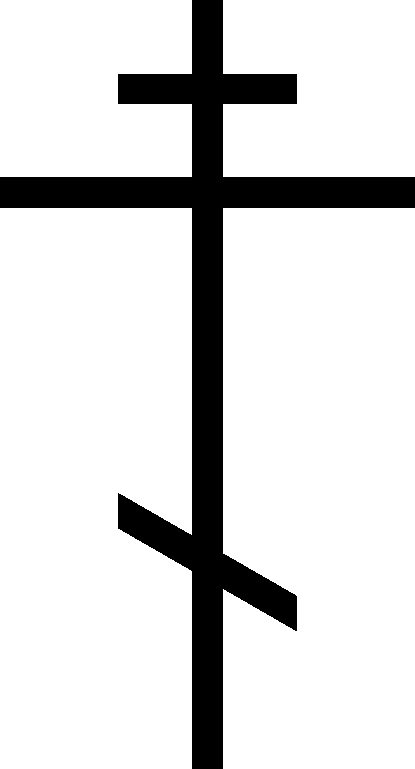
\includegraphics[height=0.4\textheight]{../back-cross.pdf}
\end{figure}

\end{document}
